\chapter{State of the art}
This chapter is about the state of the art.

\section{Theory}
This section is about the theory, for example dynamics and underactuated control.

\subsection{Underactuated system}
According to newtons second law(\( F = ma \)), The dynamics of mechanical systems can be discribed as follows:
\begin{align}
    \ddot{q} = f(q, \dot{q}, u, t)
\end{align}

Where the state is given by a vector of positions(also known as the configuration vector), and a vector of velocities, \( \dot{q}\).

For control, the second order differential equation can be rewritten as below:

\begin{align}
    \ddot{q} = f_1(q, \dot{q}, t) + f_2(q, \dot{q}, t)u
\end{align}

For a controlled dynamical system described by equation(2.2), if we have:

\begin{align}
    \text{rank}[f_2(q, \dot{q}, t)] < \text{dim}[q]
\end{align}

then the system is underactuated at \((q, \dot{q}, t)\). There is another case for underactuation is even when \(f_2\) is full rank, but additional constraints like \(|\mathbf{u}| \leq 1\) can also make a system underactuated.


\subsection{Dynamics of underactuated double pendulum system}
As shown in figure 2.1, we model the dynamics of the double pendulum with 15 parameters which include 8 link parameters namely masses \((m_1,m_2)\)
, lengths \((l_1,l_2)\)
, center of masses \((r_1,r_2)\) 
, inertias \((I_1,I_2)\)
 for the two links, and 6 actuator parameters namely motor inertia \(I_r\)
, gear ratio \(g_r\)
, coulomb friction \((c_{f1},c_{f2})\)
, viscous friction \((b_1,b_2)\)
 for the two joints and gravity.
\begin{figure}[h]
  \centering
  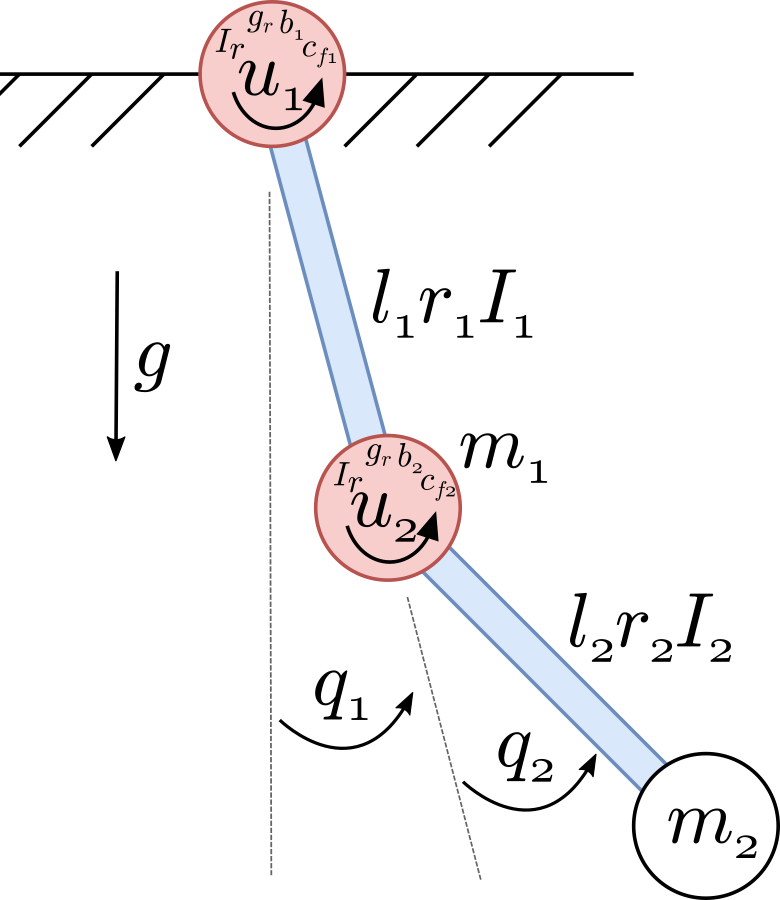
\includegraphics[width=0.5\textwidth]{figures/double_pendulum_dynamics.png} % Replace "example-image" with the actual image file name and path
  \caption{Double pendulum dynamics}
  \label{fig:sample}
\end{figure}

The generalized coordinates \( \mathbf{q} =(q_1,q_2)^T \) are the joint angles measured from the free hanging position. The state vector of the systems contains the position coordinates and their time derivatives: \(\mathbf{x}=(\mathbf{q},\mathbf{\dot{q}})^T\). The torque applied by the actuators are \(\mathbf{u}=(u_1,u_2)\). The equation of motion for the dynamics of a dynamical system can be derived following the blow steps:

\textbf{Step 1. Define the Lagrangian (\(L\)):}

   The Lagrangian (\(L\)) is defined as the difference between the kinetic energy (\(T\)) and the potential energy (\(U\)) of the system:
   \begin{align}
         L = T - U
   \end{align}


\textbf{Step 2. Express the Kinetic Energy (\(T\)):}

   The kinetic energy (\(T\)) of the double pendulum is the sum of the kinetic energies of both pendulums. The kinetic energy for a pendulum is given by:
   \begin{align}
        T = \frac{1}{2} m_1 (\dot{x}_1^2 + \dot{y}_1^2) + \frac{1}{2} m_2 (\dot{x}_2^2 + \dot{y}_2^2)
   \end{align}

   where \(m_1\) and \(m_2\) are the masses of the pendulums, \((x_1, y_1)\) and \((x_2, y_2)\) are their positions, and \(\dot{x}_1, \dot{y}_1, \dot{x}_2, \dot{y}_2\) are their respective velocities.

\textbf{Step 3. Express the Potential Energy (\(U\)):}

   The potential energy (\(U\)) of the double pendulum is the sum of the potential energies of both pendulums. The potential energy for a pendulum in a gravitational field is given by:
   \begin{align}
         U = m_1 g y_1 + m_2 g y_2
   \end{align}

   where \(g\) is the acceleration due to gravity.
   
   
\textbf{Step 4. Formulate the Lagrange's Equation:}

   Use Lagrange's equation to derive the equations of motion for the generalized coordinates \(x_1, y_1, x_2, y_2\).

    \begin{align}
    \frac{d}{dt} \left(\frac{\partial L}{\partial \dot{q_i}}\right) - \frac{\partial L}{\partial q_i} = 0
    \end{align}

\textbf{Step 5. Solve the Equations of Motion:}

   Solve the obtained set of second-order differential equations to determine the equations of motion for the system. The system dynamics with friction is:
   
   \begin{align}
        M(q)\ddot{q} + C(q,\dot{q})\dot{q} &= Du + G(q) - F(\dot{q})
   \end{align}
    
    Because the state vector is \(\mathbf{x}=(\mathbf{q},\mathbf{\dot{q}})^T\), the equation of motion can also be expressed as:
    
    \begin{equation}
    \begin{split}
        \dot{x} &= f(x,u) \\
        &= \begin{bmatrix} 
            \dot{q} \\ 
            M^{-1}(Du - C(q,\dot{q})\dot{q} + G(q) - F(\dot{q})) 
       \end{bmatrix}
    \end{split}
    \end{equation}

   Consider the forward kinematics of double pendulum system, the coordinate of the joint between the first link and the second link is \(P_1=(x_1,y_1)\),the coordinate of the end effector is \(P_2=(x_2,y_2)\).

    \begin{align}
        \label{eq:first_set}
        \left\{
        \begin{aligned}
        x_1 &= l_1 \sin(q_1) \\
        y_1 &= - l_1 \cos(q_1)
        \end{aligned}
        \right.
    \end{align}

    \begin{align}
        \label{eq:second_set}
        \left\{
        \begin{aligned}
        x_2 &= l_1 \sin(q_1) + l_2 \sin(q_1 + q_2) \\
        y_2 &= -l_1 \cos(q_1) - l_2 \cos(q_1 + q_2)
        \end{aligned}
        \right.
    \end{align}

    Put equation(2.12) and (2.13) into (2.7)(2.8)(2.9)(2.10),we can get the mass matrix (with \(s_1 = \sin(q_1), c_1 = \cos(q_1), \ldots\))
    \begin{equation}
    \mathbf{M} =
    \left[ 
    {\begin{array}{cc}
    I_1 + I_2 + l_1^2m_2 + 2l_1m_2r_2c_2 + g_r^2I_r + I_r  &   I_2 + l_1m_2r_2c_2 - g_rI_r  \\
    I_2 + l_1m_2r_2c_2 - g_rI_r                    & I_2 + g_r^2I_r                       \\
    \end{array}} 
    \right]
    \end{equation}
    
    the Coriolis matrix:
    \begin{equation}
    \begin{split}
    \mathbf{C} = \left[
    \begin{matrix}
    -2 \dot{q}_2 l_{1} m_{2} r_{2} \sin(q_2) & -\dot{q}_2 l_{1} m_{2} r_{2} \sin(q_2)\\
    \dot{q}_1 l_{1} m_{2} r_{2} \sin(q_2) & 0
    \end{matrix}
    \right],
    \label{eq:coriolis_matrix}
    \end{split}
    \end{equation}
    
    The gravity vector:
    \begin{equation}
    \begin{split}
    \mathbf{G} = \left[
    \begin{matrix}
    - g m_{1} r_{1} \sin(q_1) - g m_{2} \left(l_{1} \sin(q_1) + r_{2} \sin(q_{1+2}) \right) \\
    - g m_{2} r_{2} \sin(q_{1+2})
    \end{matrix}
    \right],
    \label{eq:gravity_matrix}
    \end{split}
    \end{equation}
    
    The friction vector:
    \begin{equation}
        \begin{split}
            \mathbf{F} =
            \left[
                \begin{matrix}
                    b_1 \dot{q}_1 + c_{f1} \arctan(100\,\dot{q}_1) \\
                    b_2 \dot{q}_2 + c_{f2} \arctan(100\,\dot{q}_2)
                \end{matrix}
            \right]
        \end{split}
    \end{equation}
    (the \(\arctan(100\,\dot{q}_i)\) function is used to approximate the discrete step function for the coulomb friction)

    and the actuator selection matrix \(\mathbf{D}\):
    \begin{equation}
        \begin{split}
            \mathbf{D}_{full} =
            \left[
                \begin{matrix}
                    1 & 0 \\
                    0 & 1
                \end{matrix}
            \right],
            \quad
            \mathbf{D}_{pendu} =
            \left[
                \begin{matrix}
                    1 & 0 \\
                    0 & 0
                \end{matrix}
            \right],
            \quad
            \mathbf{D}_{acro} =
            \left[
                \begin{matrix}
                    0 & 0 \\
                    0 & 1
                \end{matrix}
            \right]
        \end{split}
    \end{equation}
    for the fully actuated system, the pendubot or the acrobot.

\section{Related work}
In this section, we want to introduce the methods of underactuated control and the works related.

\subsection{Feedback cancellation}
Fully actuated systems are dramatically easier to control than underactuated systems. For fully actuated systems with accurate, known dynamics(e.g. \(f_1\) and \(f_2\) are known for a second order system), it is possible to use feedback to effectively change an arbitrary control problem into the problem of controlling a simple linear system.

When \(f_2\) has full row rank, it is invertible. Consider the potential nonlinear feedback control:

\begin{align}
 u = \pi(q, \dot{q}, t) = f_2^{-1}(q, \dot{q}, t) [u' - f_1(q, \dot{q}, t)]
\end{align}

where \(u'\) is the new control input(can be viewed as an internal input into your controller). Applying this feedback controller to equation(2.2) can lead to a linear, decoupled, second order system.

\begin{align}
  \ddot{q} = u' 
\end{align}

In other words, if \(f_1\) and \(f_2\) are known and \(f_2\) is invertible, the system is "feedback equivalent" to \(\ddot{q} = u' \). Then we can use simple control method for linear systems to handle is equivalent system.

\subsection{PFL:Partial Feedback Linearization}

\subsection{Energy shaping}
example: torque limited simple pendulum

\subsection{Reinforcement-Learning based control}
Something about model free reinforcement learning and model based reinforcement learning.


\cleardoublepage
